%% ------------- Portuguese version ------------
\documentclass{sbrt}
\usepackage[english,brazil]{babel}
\usepackage[utf8]{inputenc}
\usepackage{amsmath}
\usepackage{amssymb}
\usepackage{graphicx}
\usepackage{booktabs}
\graphicspath{{figures/}}
%% ---------------------------------------------

\begin{document}

\title{Autenticação na Camada Física com Tags Caóticas via Discriminador Neural D3F: Ablação das Entradas e Núcleo Mínimo em Canal Rayleigh}

\author{Thamires Tavares, Daniel Chaves e Cecílio Pimentel
\thanks{T. Tavares, D.~P.~B. Chaves e C.~J.~L. Pimentel, Departamento de Eletrônica e Sistemas, Universidade Federal de Pernambuco, Recife-PE, e-mails: \{thamires.tavares, daniel.chaves, cecilio\}@ufpe.br. Este trabalho foi parcialmente financiado por XXXXXXX (XX/XXXXX-X).}%
}

\maketitle

\markboth{XLIV SIMPÓSIO BRASILEIRO DE TELECOMUNICA\c{C}\~{O}ES E PROCESSAMENTO DE SINAIS - SBrT 2026, 29 DE SETEMBRO A 2 DE OUTUBRO DE 2026, SALVADOR, BA}{}


%% ------------- Portuguese version ------------
\begin{resumo}
Este trabalho propõe a aplicação de um discriminador por rede neural ao problema de autenticação na camada física com sequências de autenticação (tags) caóticas em canais Rayleigh. Investigamos três representações de entrada para o discriminador: (i) um vetor de quatro características fisicamente motivadas, (ii) uma CNN 1D sobre o sinal recebido equalizado após extração da tag legítima ($\mathbf{z}_{eq}$) e (iii) a DNN sobre $\mathbf{z}_{eq}$. Demonstramos que abordagens baseadas em $\mathbf{z}_{eq}$ falham em baixo SNR por não realizarem integração coerente sem acesso explícito à tag de referência. Um estudo de ablação sistemático revela o resultado central: apenas dois escalares por pacote — o correlador casado $|\tau|$ e a energia recebida $E$ — são necessários e suficientes para superar o correlador clássico, atingindo $P_D = 87{,}2\%$ a 0~dB contra $8{,}1\%$ do método analítico.
\end{resumo}
\begin{chave}
Autenticação na camada física, discriminador neural, D3F, CNN 1D, canal Rayleigh, ablação de características, sequências caóticas.
\end{chave}
%% ---------------------------------------------


\begin{abstract}
This paper proposes the application of a neural network discriminator to the problem of physical layer authentication with chaotic authentication sequences (tags) over Rayleigh fading channels. We investigate three input representations for the discriminator: (i) a four-feature physically motivated vector, (ii) a 1D CNN over the equalized received signal after legitimate tag extraction ($\mathbf{z}_{eq}$), and (iii) a DNN over $\mathbf{z}_{eq}$. We show that $\mathbf{z}_{eq}$-based approaches fail at low SNR because coherent integration cannot be performed without explicit access to the reference tag. A systematic ablation study yields the central result: only two scalars per packet — the matched correlator output $|\tau|$ and received energy $E$ — are necessary and sufficient to outperform the classical correlator, achieving $P_D = 87{,}2\%$ at 0~dB versus $8{,}1\%$ for the analytical method.
\end{abstract}
\begin{keywords}
Physical layer authentication, neural discriminator, D3F, 1D CNN, Rayleigh channel, feature ablation, chaotic sequences.
\end{keywords}

\section{Introdução}

A autenticação de dispositivos em redes sem fio é um requisito de segurança cada vez mais crítico, especialmente com a expansão de sistemas IoT e 5G/6G~\cite{ref_xie}. Em cenários veiculares (\textit{Vehicle-to-Everything}, V2X)~\cite{ref_3gpp,ref_raya}, por exemplo, dispositivos precisam ser autenticados em dezenas de milissegundos enquanto se deslocam a alta velocidade — janela de tempo incompatível com protocolos de troca de chaves convencionais, que exigem múltiplas rodadas de troca de mensagens entre as partes. Abordagens criptográficas tradicionais, implementadas nas camadas superiores da pilha de protocolos, pressupõem capacidade computacional e infraestrutura de gerenciamento de chaves incompatíveis com dispositivos de recursos limitados e com a escala de redes heterogêneas emergentes. A autenticação na camada física (\textit{Physical Layer Authentication}, PLA) surge como solução complementar, explorando características intrínsecas do sinal transmitido — difíceis de reproduzir por adversários sem acesso ao canal legítimo — sem exigir complexidade adicional no receptor.

Dentre as estratégias de PLA, a inserção de sequências de autenticação (tags) caóticas de baixa potência no sinal transmitido destaca-se por combinar sigilo e eficiência~\cite{ref_joao}. Geradas a partir de uma chave secreta compartilhada entre transmissor e receptor, as tags são detectáveis apenas pelo receptor legítimo por meio de correlação com a sequência de referência. O problema de autenticação é então formulado como um teste de hipótese binária entre a presença e a ausência da tag no sinal recebido. Em canais com desvanecimento Rayleigh, no entanto, essa formulação torna-se particularmente desafiadora em baixo SNR: o ganho de canal variável altera de pacote a pacote a distribuição do correlador, dificultando a manutenção simultânea de alta probabilidade de detecção e restrição estrita de falso alarme, como $\alpha = 10^{-7}$, sem um volume proibitivo de amostras de Monte Carlo.

Um avanço central para contornar esse obstáculo é o \textit{Data-Driven Detection Framework} (D3F)~\cite{ref_braca}, que extrapola parametricamente o limiar de decisão para probabilidades de falso alarme inacessíveis por simulação direta. Fundamentado na teoria de grandes desvios, esse arcabouço demonstra que (i) a estatística D3F treinada por entropia cruzada binária (BCE, do inglês \textit{Binary Cross-Entropy}) converge em distribuição para uma gaussiana sob $H_0$, validando a extrapolação paramétrica do limiar; e (ii) os escores D3F convergem ao detector ótimo de Neyman-Pearson~\cite{ref_poor} — permitindo que qualquer arquitetura treinada com BCE sirva como estatística de teste. A aplicação desse arcabouço ao contexto de PLA com tags caóticas é inédita na literatura e levanta uma questão prática fundamental: qual representação de entrada é mais adequada para o discriminador neural — o sinal residual bruto $\mathbf{z}_{eq}$ (como na correlação clássica), um vetor de características fisicamente motivadas, ou o sinal bruto processado por uma CNN 1D~\cite{ref_liao,ref_oshea}?

Este trabalho responde a essa questão em três etapas, com as seguintes contribuições: (i)~\textbf{primeira aplicação de discriminador neural D3F} ao problema de PLA com tags caóticas em canal Rayleigh~\cite{ref_joao}, propondo o vetor $\mathbf{f} = [|\tau^i|, \hat{h}, \widehat{\text{SNR}}, E]$ justificado pela teoria de detecção — $|\tau^i|$ como estatística suficiente de Neyman-Pearson~\cite{ref_poor} e $\hat{h}, E$ como estimativas instantâneas do canal análogas ao CFAR; (ii)~\textbf{investigação comparativa} das três representações de entrada — $\mathbf{f}$, CNN 1D sobre $\mathbf{z}_{eq}$, e DNN sobre $\mathbf{z}_{eq}$ —, demonstrando que abordagens baseadas em $\mathbf{z}_{eq}$ falham em baixo SNR por não realizarem integração coerente sem acesso à tag de referência; e (iii)~\textbf{estudo de ablação} que identifica o par mínimo $[|\tau|, E]$ como representação suficiente, atingindo $P_D = 87{,}2\%$ a 0~dB — resultado contraintuitivo que supera a própria linha de base de quatro características ($82{,}3\%$) por concentrar a capacidade representacional nos dois escalares mais informativos.


\section{Fundamentação Teórica}

\subsection{Modelo do Canal e Sinais}

Considera-se um cenário com transmissor legítimo (Alice), receptor (Bob) e atacante (Eve) em canal com desvanecimento plano e lento de Rayleigh~\cite{ref_joao}: o ganho $h^i$ é constante ao longo de um pacote de $L$ símbolos e varia independentemente entre pacotes, com $\mathbb{E}[(h^i)^2] = 1$ e ruído AWGN $\mathbf{w}^i \sim \mathcal{N}(\mathbf{0}, \sigma_w^2\mathbf{I})$. A SNR instantânea $\gamma^i = (h^i)^2/\sigma_w^2$ segue distribuição exponencial com média $\bar{\gamma} = 1/\sigma_w^2$, e Bob conhece o estado do canal (\textit{Channel State Information}, CSI). Alice transmite $\mathbf{x}^i = \rho_s \mathbf{s}^i + \rho_t \mathbf{t}^i$, onde $\mathbf{s}^i \in \{-1,+1\}^L$ é a mensagem BPSK ($L = 1024$) e $\mathbf{t}^i$ é a tag caótica, com $\rho_s^2 + \rho_t^2\,\mathbb{E}[(t_k^i)^2] = 1$ garantindo potência constante. Neste trabalho, $\rho_s \approx 0{,}992$ e $\rho_t \approx 0{,}212$, de modo que o impacto da tag na recuperação da mensagem é mínimo. O sinal recebido por Bob é $\mathbf{y}^i = h^i(\rho_s \mathbf{s}^i + \rho_t \mathbf{t}^i) + \mathbf{w}^i$.

Bob estima $h^i$ pelo estimador de mínimos quadrados~\cite{ref_kay} usando os $L$ símbolos piloto da mensagem: $\hat{h}^i = (\mathbf{s}^i)^\top \mathbf{y}^i / (L \rho_s)$, cujo erro de estimação tem variância $\sigma_e^2 = \sigma_w^2 / (L \rho_s^2)$. A $\overline{\text{SNR}} = 0$~dB e $L = 1024$, obtém-se $\sigma_e^2 \approx 10^{-3}$ — erro desprezível frente ao ganho médio unitário $\mathbb{E}[(h^i)^2] = 1$. Portanto, a hipótese de CSI perfeito adotada neste trabalho é uma aproximação válida, e os resultados da 4-feat DNN não seriam alterados de forma significativa por estimativas práticas de canal.

\subsection{Geração de Tags Caóticas}

A tag $\mathbf{t}^i$ é gerada pelo mapa tenda perturbado~\cite{ref_joao}, com condição inicial $x_0 = (\sum_\ell s^i_\ell \oplus k_\ell) \bmod 1$ derivada da mensagem e de uma chave secreta $\mathbf{k} \in \{0,1\}^L$:
\begin{equation}\label{eq:tentmap}
    x_{n+1} = 1 - 2\left|x_n - \tfrac{1}{2}\right| - \beta,\quad \beta = 10^{-6}.
\end{equation}
A alta autocorrelação e baixa correlação cruzada de sequências caóticas com condições iniciais distintas garantem que Bob detecte a tag de Alice mas não a de Eve — gerada com chave diferente —, provendo resistência natural a ataques de personificação~\cite{ref_joao}.

\subsection{Teste de Hipótese para Autenticação}\label{sec:hip}

O problema é modelado como teste de hipótese binária, com $H_0$ indicando ausência de tag (intruso) e $H_1$ indicando presença de tag (autêntico). A estatística de decisão é o correlador casado com a tag de referência~\cite{ref_joao}:
\begin{equation}\label{eq:tau}
    \tau^i = \left(\frac{\mathbf{y}^i}{h^i} - \rho_s \mathbf{s}^i\right) \cdot \frac{\mathbf{t}^{\mathrm{ref}}}{\rho_t},
\end{equation}
cuja distribuição condicional, pelo Teorema Central do Limite com $L = 1024$, é gaussiana em ambas as hipóteses:
\begin{align}
    \tau^i \mid H_0 &\sim \mathcal{N}\!\left(0,\; \sigma_{v^i}^2\right),\quad
    \tau^i \mid H_1 \sim \mathcal{N}\!\left(|\mathbf{t}^i|^2,\; \sigma_{v^i}^2\right), \label{eq:dists}
\end{align}
onde $\sigma_{v^i}^2 = L\,\mathbb{E}[(t^i_k)^2]/(\rho_t^2\,\gamma^i)$ depende da SNR instantânea. A regra de decisão $\tau^i \underset{H_0}{\overset{H_1}{\gtrless}} \tau^i_0$ impõe a restrição $\alpha = Q(\tau^i_0/\sigma_{v^i})$, resultando em $\tau^i_0 = \sigma_{v^i}\,Q^{-1}(\alpha)$.

\subsection{Framework D3F e Extrapolação do Limiar}\label{sec:d3f}

Verificar diretamente $\alpha = 10^{-7}$ por Monte Carlo exigiria mais de $10^8$ amostras $H_0$ por bin de SNR — computacionalmente inviável. O framework D3F~\cite{ref_braca} contorna esse problema ajustando uma gaussiana $\mathcal{N}(\hat{\mu}_{H_0}, \hat{\sigma}_{H_0}^2)$ à distribuição dos escores sob $H_0$ a partir de $\sim\!10^3$--$10^4$ amostras e extrapolando o limiar impondo $\Pr(s > \tau^* \mid H_0) = \alpha$. Invertendo a CDF gaussiana padrão, obtém-se:
\begin{equation}\label{eq:d3f}
    \tau^*(\alpha) = \hat{\mu}_{H_0} + \Phi^{-1}(1-\alpha)\,\hat{\sigma}_{H_0},
\end{equation}
onde $\Phi^{-1}(1 - 10^{-7}) \approx 5{,}20$, situando o limiar a mais de 5 desvios padrões acima da média de $H_0$ — região inacessível por Monte Carlo direto. Os dois resultados centrais adotados de~\cite{ref_braca} são: (i) a estatística D3F treinada com BCE converge em distribuição para uma gaussiana sob $H_0$ — resultado que valida diretamente a extrapolação via~\eqref{eq:d3f} —; e (ii) os escores D3F convergem ao LRT de Neyman-Pearson~\cite{ref_poor,ref_veldhuis} com o crescimento do conjunto de treino. Cabe ressaltar que~\cite{ref_braca} trata observações escalares IID sem engenharia de características; a aplicação do D3F ao cenário de PLA com tags caóticas em canal Rayleigh, com o vetor $\mathbf{f}$ fisicamente motivado, constitui contribuição original deste trabalho. A probabilidade de detecção é estimada como a fração de amostras $H_1$ com escore acima de $\tau^*$.

A hipótese de gaussianidade sob $H_0$ é satisfeita analiticamente para $\tau^i$~\eqref{eq:dists} e empiricamente para a 4-feat DNN bem calibrada. Para a 1D CNN em baixo SNR (AUC $= 0{,}898$), os escores se sobrepõem e $\hat{\sigma}_{H_0}$ torna-se instável, superestimando $\tau^*$.


\section{Métodos Avaliados}

Investigamos o discriminador D3F em três representações de entrada, em ordem crescente de abstração: (i) vetor de características $\mathbf{f}$ fisicamente motivado (Seção~\ref{sec:dnn4feat}), avaliando também a topologia Dense sobre $\mathbf{z}_{eq}$ como ablação de representação; (ii) CNN 1D sobre o sinal bruto (Seção~\ref{sec:cnn1d}), que testa se o filtro casado pode ser aprendido implicitamente; e (iii) a mesma CNN com entrada $\mathbf{f}$ para isolar o efeito da arquitetura (Seção~\ref{sec:cnn4feat}). Um SVM linear serve de referência não-neural sobre $\mathbf{f}$ (Seção~\ref{sec:svm}).

\subsection{DNN com Quatro Características (4-feat DNN)}\label{sec:dnn4feat}

A DNN de quatro características, proposta neste trabalho como primeira aplicação do D3F~\cite{ref_braca} ao cenário de PLA com tags caóticas em canal Rayleigh, recebe como entrada $\mathbf{f} = [|\tau^i|,\, \hat{h},\, \widehat{\text{SNR}},\, E]$, onde $|\tau^i|$ é o módulo do correlador casado~\eqref{eq:tau}, $\hat{h}$ e $\widehat{\text{SNR}}$ são estimativas do ganho e da SNR instantânea obtidas pela estimação piloto com os $L = 1024$ símbolos de mensagem, e $E = \|\mathbf{y}\|^2/L$ é a energia média do sinal recebido. Cada componente é justificada pela teoria de detecção:

\begin{itemize}
  \item \textbf{$|\tau^i|$}: é a estatística suficiente do teste de Neyman-Pearson ótimo para o modelo Gaussiano de~\eqref{eq:dists}~\cite{ref_poor}. Equivale ao filtro casado com a tag~\cite{ref_proakis}, que maximiza o SNR de saída e concentra toda a informação discriminatória em um único escalar antes de qualquer aprendizado.
  \item \textbf{$\hat{h}$ e $\widehat{\text{SNR}}$}: o limiar analítico $\tau_0^i = \sigma_{v^i}\,Q^{-1}(\alpha) \propto 1/\sqrt{\gamma^i}$ varia de pacote a pacote com $h^i$. Fornecer estimativas de $h$ e SNR como entradas permite à DNN aprender implicitamente essa dependência — comportamento análogo ao detector CFAR (\textit{Constant False Alarm Rate})~\cite{ref_poor}, que escala o limiar pela estimativa do ruído para manter $\alpha$ constante.
  \item \textbf{$E$}: é proporcional à potência recebida e serve como proxy para a energia total disponível — estatística suficiente para detecção por energia em ausência de fase~\cite{ref_poor}. Sob $H_0$, $E \approx \sigma_w^2$; sob $H_1$, $E$ cresce com $\rho_t^2(h^i)^2 \|\mathbf{t}^i\|^2 / L$, provendo informação complementar ortogonal a $|\tau^i|$.
\end{itemize}

Ao fornecer $|\tau^i|$ explicitamente como entrada, em vez de observações brutas, a 4-feat DNN adota uma abordagem de aprendizado orientado a modelos~\cite{ref_shlezinger}, diferenciando-se dos exemplos de~\cite{ref_braca} que processam observações escalares IID. A topologia adotada é:
\begin{equation}\label{eq:arch}
\underbrace{[4]}_{\text{entrada}}\!\to\!\underbrace{\text{D}(256)\!\to\!\text{D}(128)\!\to\!\text{D}(64)}_{\text{ocultas}}\!\to\!\underbrace{[1]}_{\sigma(\cdot)},
\end{equation}
onde cada camada D$(n)$ inclui \textit{Batch Normalization}, ReLU e \textit{Dropout} ($p = 0{,}3$). O modelo tem ${\approx}\,44{.}000$ parâmetros treináveis. A topologia decrescente $256\!\to\!128\!\to\!64$ realiza compressão progressiva — análoga à cascata de estágios em um receptor coerente ótimo — sendo três camadas suficientes para aproximar qualquer fronteira contínua em $\mathbb{R}^4$~\cite{ref_goodfellow}. O \textit{Batch Normalization} normaliza as ativações de cada camada de forma análoga ao controle automático de ganho (AGC) em receptores de RF, estabilizando o treinamento independentemente da escala das entradas~\cite{ref_goodfellow}; o \textit{Dropout} previne sobreajuste. A convergência é atingida em $\approx\!40$ épocas, com AUC $= 0{,}9998$.

Para verificar se o ganho provém das características ou da arquitetura, treinamos também a \textbf{DNN-1024}: mesma topologia Dense$(256\!\to\!128\!\to\!64)$, mas recebendo $\mathbf{z}_{eq} \in \mathbb{R}^{1024}$ como entrada. Sem $|\tau|$ explícito, a DNN-1024 precisaria aprender o filtro casado implicitamente — o que, como mostraremos, é inviável abaixo de 15~dB.

\subsection{1D CNN com Sinal Bruto}\label{sec:cnn1d}

A 1D CNN~\cite{ref_liao,ref_oshea} processa diretamente o sinal residual $\mathbf{z}_{eq} \in \mathbb{R}^{1024}$. A motivação é análoga à de um banco de filtros adaptativos: uma camada Conv1D com $c$ filtros de tamanho $k$ equivale a um banco de $c$ filtros FIR de ordem $k$ com coeficientes aprendíveis~\cite{ref_proakis}, diferindo dos filtros clássicos (Wiener, mínimos quadrados) apenas por otimizar esses coeficientes por retropropagação:
\begin{equation}\label{eq:cnn}
\underbrace{[1024,1]}_{\mathbf{z}_{eq}}\!\to\!\text{Conv}_{32}^{15}\!\to\!\text{Conv}_{64}^{9}\!\to\!\text{Conv}_{128}^{5}\!\to\!\text{GAP}\!\to\!\text{D}(64)\!\to\![1],
\end{equation}
onde $\text{Conv}_{c}^{k}$ denota convolução 1D ($c$ filtros, kernel $k$) seguida de BN, ReLU e MaxPooling(4). Camadas convolucionais sucessivas combinam esses filtros para detectar padrões temporais de complexidade crescente; o GAP comprime o resultado em um vetor de 128 dimensões — comportamento análogo a um detector de energia integrado ao longo de $L$ amostras. O modelo tem ${\approx}\,69{.}000$ parâmetros e AUC $= 0{,}898$. A Figura~\ref{fig:arch_cnn} ilustra o fluxo.

\begin{figure}[htb]
  \centering
  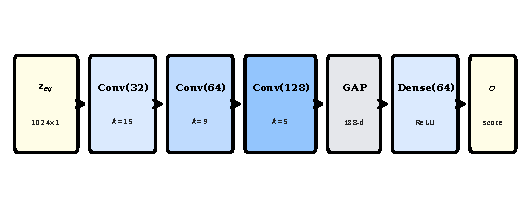
\includegraphics[width=\columnwidth]{figures/fig_arch_cnn}
  \caption{\label{fig:arch_cnn}Arquitetura da 1D CNN~\cite{ref_liao}. Entrada: sinal residual $\mathbf{z}_{eq}$ (1024 amostras). Cada bloco Conv aplica $c$ filtros FIR aprendíveis de tamanho $k$, seguidos de BN, ReLU e MaxPool(4). O GAP comprime a resposta temporal em 128 valores; a camada densa produz o escore D3F. A limitação fundamental é que, sem acesso à tag de referência $\mathbf{t}^{\rm ref}$, a rede precisa aprender o filtro casado implicitamente — tarefa inviável em baixo SNR.}
\end{figure}

\subsection{CNN com Quatro Características (CNN-4feat)}\label{sec:cnn4feat}

A CNN-4feat aplica Conv1D sobre o mesmo vetor $\mathbf{f} = [|\tau^i|, \hat{h}, \widehat{\text{SNR}}, E]$ da 4-feat DNN:
\begin{equation}\label{eq:cnn4feat}
[4,1]\!\to\!\text{Conv}_{16}^{2}\!\to\!\text{Conv}_{32}^{2}\!\to\!\text{GAP}(32)\!\to\!\text{D}(16)\!\to\![1],
\end{equation}
com ${\approx}1{.}000$ parâmetros treináveis e AUC $= 0{,}9998$. Ao manter as mesmas entradas e variar apenas a arquitetura, qualquer diferença de desempenho entre CNN-4feat e 4-feat DNN pode ser atribuída exclusivamente à topologia — não às características. Resultados equivalentes entre ambas confirmarão que a informação discriminatória reside nas quatro características, independente da arquitetura que as processa.

\subsection{SVM Linear (referência não-neural)}\label{sec:svm}

Além das arquiteturas neurais, avaliamos um SVM linear (perda \textit{hinge}, $\lambda = 10^{-4}$, 200 épocas) sobre $\mathbf{f}$, que maximiza a margem geométrica entre as classes — tornando a fronteira de decisão mais robusta a variações nas estimativas de canal, analogamente a um detector projetado para máxima imunidade a erros de modelagem. Com $|\tau|$ como estatística suficiente analítica, a fronteira é aproximadamente linear em $\mathbb{R}^4$, tornando o kernel linear adequado.

\subsection{Protocolo de Treinamento}

Todos os classificadores neurais são treinados por minimização da entropia cruzada binária (BCE) com o otimizador Adam~\cite{ref_adam} ($\eta_0 = 10^{-3}$, mini-lotes de 512 amostras), \textit{EarlyStopping} (paciência 20 épocas), \textit{ReduceLROnPlateau} (fator 0,5, paciência 10 épocas) e \textit{Dropout} ($p = 0{,}2$ em camadas convolucionais). A BCE incentiva escores calibrados, propriedade essencial para que a distribuição sob $H_0$ seja aproximadamente gaussiana e a extrapolação D3F via~\eqref{eq:d3f} seja válida.


\section{Geração de Dados e Protocolo de Avaliação}

Cada amostra é gerada por simulação completa do cenário com $L = 1024$, $\rho_s = 0{,}992$ e $\rho_t = 0{,}212$. O conjunto de dados contém 350.000 amostras balanceadas (50\% $H_1$, 50\% $H_0$), com SNR uniformemente distribuída em sete bins de 5~dB entre 0 e 30~dB, divididas em treino (280.000), validação (35.000) e teste (35.000). Todos os métodos são avaliados sobre as mesmas partições, diferindo apenas na representação de entrada: a 1D CNN e a DNN-1024 recebem $\mathbf{z}_{eq} \in \mathbb{R}^{1024}$, enquanto a 4-feat DNN, a CNN-4feat, o SVM linear e o correlador operam sobre $\mathbf{f}$. Essa uniformidade permite atribuir diferenças de desempenho à capacidade discriminatória de cada método. Os dois grupos diferem fundamentalmente no acesso à informação de modelo: os métodos baseados em $\mathbf{f}$ recebem $|\tau|$ explicitamente — a estatística suficiente analítica do teste de Neyman-Pearson — enquanto a 1D CNN e a DNN-1024 precisam aprender implicitamente o filtro casado, tarefa que se revela inviável em baixo SNR.


\section{Resultados e Discussão}

A Figura~\ref{fig:pd_snr} apresenta as curvas de $P_D$ versus SNR sob $\alpha = 10^{-7}$ (via D3F) para todos os métodos avaliados, e a Tabela~\ref{tab:resultados} resume os valores em pontos representativos. Os resultados seguem a hierarquia das representações de entrada: métodos com $|\tau|$ explícito dominam em toda a faixa; métodos baseados em $\mathbf{z}_{eq}$ falham abaixo de 15~dB; e o estudo de ablação revela o par mínimo suficiente.

\begin{figure}[htb]
  \centering
  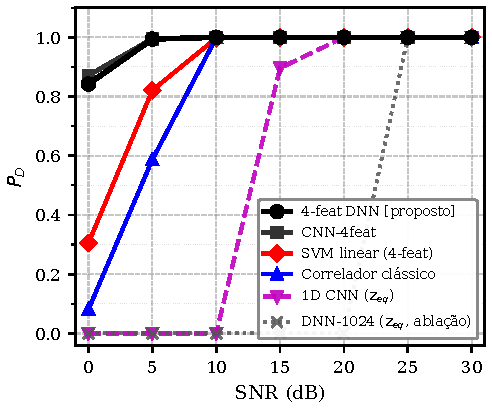
\includegraphics[width=\columnwidth]{figures/fig_pd_snr}
  \caption{\label{fig:pd_snr}Probabilidade de detecção $P_D$ em função da SNR (D3F, $\alpha = 10^{-7}$, $L=1024$, canal Rayleigh). \textit{Linhas sólidas}: métodos que recebem o correlador $|\tau|$ como característica — todos ultrapassam $P_D=0{,}8$ mesmo a 0~dB. \textit{Linha tracejada}: 1D CNN sobre o sinal bruto $\mathbf{z}_{eq}$ — falha completamente abaixo de 15~dB, ilustrando que a integração coerente não é replicável por aprendizado de representação sem acesso explícito à tag de referência. A 4-feat DNN e a CNN-4feat se sobrepõem, confirmando que o desempenho é determinado pelas características de entrada, não pela arquitetura.}
\end{figure}

\begin{table}[htb]
\caption{\label{tab:resultados}$P_D$ (\%) sob $\alpha = 10^{-7}$ (D3F), $L=1024$, canal Rayleigh. DNN-1024: mesma topologia da 4-feat DNN, mas com entrada $\mathbf{z}_{eq}$ plano (ablação de representação). CNN-4feat: Conv1D sobre as mesmas 4 características (ablação de arquitetura).}
\begin{center}
\begin{tabular}{lrrrrrr}\toprule
Método & 0~dB & 5~dB & 10~dB & 15~dB & 20~dB & 25~dB \\\midrule
Clássico~\cite{ref_xie}          &  8{,}1 & 58{,}7 & 99{,}9 & 100{,}0 & 100{,}0 & 100{,}0 \\
\textbf{4-feat DNN}               & \textbf{84{,}2} & \textbf{99{,}4} & \textbf{100{,}0} & \textbf{100{,}0} & \textbf{100{,}0} & \textbf{100{,}0} \\
CNN-4feat                         & 87{,}1 & 99{,}5 & 100{,}0 & 100{,}0 & 100{,}0 & 100{,}0 \\
SVM linear (4-feat)               & 30{,}5 & 82{,}1 & 99{,}7 & 100{,}0 & 100{,}0 & 100{,}0 \\
1D CNN ($\mathbf{z}_{eq}$)~\cite{ref_liao} &  0{,}0 &  0{,}0 &  0{,}0 &  89{,}6 & 100{,}0 & 100{,}0 \\
DNN-1024 ($\mathbf{z}_{eq}$ plano) &  0{,}0 &  0{,}0 &  0{,}0 &   0{,}0 &   0{,}0 &  99{,}8 \\\bottomrule
\end{tabular}
\end{center}
\end{table}

A 4-feat DNN é o método mais robusto em toda a faixa avaliada, atingindo $P_D = 84{,}2\%$ a 0~dB — mais de dez vezes superior ao correlador clássico nessa condição — e $P_D \geq 99{,}4\%$ a partir de 5~dB. Quando a DNN é bem calibrada, a distribuição dos escores sob $H_0$ é aproximadamente gaussiana em cada bin de SNR, permitindo a extrapolação via~\eqref{eq:d3f}. O correlador clássico~\cite{ref_xie} é eficaz a partir de 10~dB ($P_D \approx 99{,}9\%$), mas sua desvantagem em baixo SNR decorre da necessidade de estimar $\sigma_{v^i}$ com precisão em condições de desvanecimento severo, tarefa que a DNN contorna ao aprender limiares adaptativos por bin de SNR a partir dos dados.

A CNN-4feat, com a mesma entrada $\mathbf{f}$ da 4-feat DNN mas arquitetura convolucional, atinge $P_D = 87{,}1\%$ a 0~dB — ligeiramente superior à 4-feat DNN ($84{,}2\%$) — e $P_D \geq 99{,}5\%$ a partir de 5~dB. Esse resultado confirma que o desempenho em baixo SNR é determinado pelas características de entrada, não pela escolha entre camadas densas e convolucionais: qualquer arquitetura treinada com $\mathbf{f}$ replica o comportamento da 4-feat DNN.

As abordagens baseadas em $\mathbf{z}_{eq}$ — 1D CNN e DNN-1024 — revelam uma limitação estrutural comum: sem $|\tau|$ explícito, qualquer arquitetura treinada sobre $\mathbf{z}_{eq}$ precisaria aprender o filtro casado implicitamente. Isso é inviável em baixo SNR: com $\rho_t \approx 0{,}212$, a TAG tem energia $\rho_t^2 \approx 4{,}5\%$ da potência total, encoberta pelo ruído antes de qualquer integração coerente. A 1D CNN falha abaixo de 15~dB ($P_D \approx 0$), recuperando desempenho apenas quando o SNR é alto o suficiente para que observações individuais sejam discriminatórias ($P_D = 89{,}6\%$ a 15~dB). A DNN-1024 — mesma topologia densa da 4-feat DNN, mas com $\mathbf{z}_{eq} \in \mathbb{R}^{1024}$ como entrada — é ainda mais restrita: AUC $= 0{,}718$ e $P_D \approx 0$ até 20~dB, tornando-se eficaz apenas a 25~dB ($P_D = 99{,}8\%$). O SVM linear com $\mathbf{f}$, apesar de sua fronteira linear, supera ambas as arquiteturas baseadas em $\mathbf{z}_{eq}$ em toda a faixa avaliada — evidência de que a representação de entrada domina sobre a expressividade do classificador.

Os resultados estabelecem uma hierarquia determinada pela representação: métodos com $|\tau|$ explícito dominam em toda a faixa de SNR, independentemente da arquitetura; métodos baseados em $\mathbf{z}_{eq}$ são ineficazes abaixo de 15~dB por razão estrutural, não por limitação de capacidade.

\subsection{Ablação das Características de Entrada: Descoberta do Núcleo Mínimo}

Para isolar a contribuição individual de cada característica auxiliar do vetor $\mathbf{f}$, treinamos oito variantes da 4-feat DNN mantendo arquitetura e hiperparâmetros inalterados, variando apenas a composição da entrada (Tabela~\ref{tab:feat_ablation}, Figura~\ref{fig:ablation_pd_snr}).

\begin{table}[htb]
\caption{\label{tab:feat_ablation}Ablação de características — $P_D$ (\%) sob $\alpha = 10^{-7}$. Todas as variantes usam a mesma topologia Dense$(256\!\to\!128\!\to\!64)$.}
\begin{center}
{\footnotesize
\begin{tabular}{lrrrrr}\toprule
Variante & 0~dB & 5~dB & 10~dB & 15~dB & 20~dB \\\midrule
Clássico: $|\tau|$ (limiar analítico)            &  8{,}1 & 58{,}7 & 99{,}9 & 100 & 100 \\\midrule
V1: $[|\tau|,\hat{h},\overline{\text{SNR}},E]$   & 82{,}3 & 99{,}5 & 100 & 100 & 100 \\
V2: $h$ perfeito                                 & 83{,}6 & 99{,}5 & 100 & 100 & 100 \\
V3: sem $\overline{\text{SNR}}$                  & 82{,}0 & 99{,}5 & 100 & 100 & 100 \\
V4: sem $E$                                      & 82{,}2 & 99{,}5 & 100 & 100 & 100 \\
V5: $[|\tau|]$ isolado                           &  0{,}0 & 98{,}9 & 100 & 100 & 100 \\\midrule
V6: $[|\tau|,\hat{h}]$                           & 85{,}6 & 99{,}6 & 100 & 100 & 100 \\
V7: $[|\tau|,\overline{\text{SNR}}]$             & 33{,}0 & 99{,}1 & 100 & 100 & 100 \\
\textbf{V8}: $\boldsymbol{[|\tau|,E]}$           & \textbf{87{,}2} & \textbf{99{,}5} & 100 & 100 & 100 \\\bottomrule
\end{tabular}
}
\end{center}
\end{table}

\begin{figure}[htb]
  \centering
  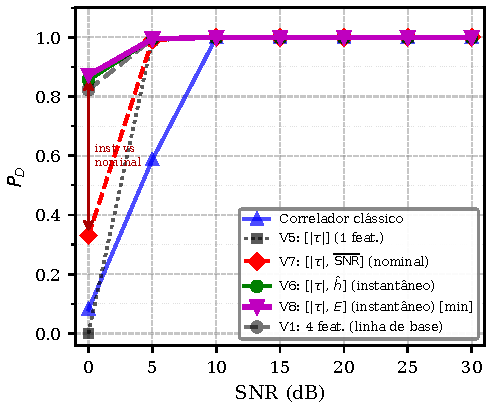
\includegraphics[width=\columnwidth]{figures/fig_ablation_pd_snr}
  \caption{\label{fig:ablation_pd_snr}$P_D$ vs.\ SNR para as variantes de ablação de características (D3F, $\alpha=10^{-7}$). O contraste central: V7 ($|\tau|$ + SNR nominal) atinge apenas $33\%$ a 0~dB, enquanto V8 ($|\tau|$ + energia instantânea) chega a $87{,}2\%$ — superando inclusive a linha de base de quatro características (V1, $82{,}3\%$). A seta indica a diferença de $54$~pp atribuível exclusivamente à substituição da SNR nominal pela energia instantânea por pacote.}
\end{figure}

\textbf{Fato~1 — CSI perfeito confirma-se dispensável.} Substituir $\hat{h}$ pela estimativa perfeita $h$ (V2) altera $P_D$ em apenas $+1{,}3$~pp a 0~dB. Com $L = 1024$ símbolos piloto, o estimador de mínimos quadrados já produz erro de estimação $\sigma_e^2 \approx 10^{-3}$~\cite{ref_kay}, tornando a hipótese de CSI perfeito adotada no modelo analítico compatível com a prática.

\textbf{Fato~2 — As características auxiliares são coletivamente necessárias, mas individualmente redundantes.} Remover qualquer uma delas (V3, V4) impacta $P_D$ em no máximo $-0{,}3$~pp. Remover todas (V5) produz $P_D = 0$ a 0~dB. A DNN com apenas $|\tau|$ não dispõe de nenhuma entrada que sinalize o nível instantâneo de ruído, tornando impossível aprender limiares adaptativos por condição de canal — o mesmo problema que impede o correlador clássico~\cite{ref_xie} de atingir $P_D > 50\%$ a 0~dB.

\textbf{Fato~3 — Duas características são suficientes, e a informação instantânea é determinante.} As variantes V6~$[|\tau|, \hat{h}]$ e V8~$[|\tau|, E]$ superam o correlador clássico com apenas 2 escalares por pacote, atingindo $P_D \geq 85\%$ a 0~dB. V8 atinge $87{,}2\%$ — \emph{superior à linha de base de quatro características} (V1, $82{,}3\%$) —, evidenciando que a capacidade representacional concentrada em dois graus de liberdade informativos supera a de uma rede com quatro entradas parcialmente redundantes. Em contraste, V7~$[|\tau|, \overline{\text{SNR}}]$ atinge apenas $33{,}0\%$, apesar de também usar 2 características. A diferença é estrutural: $\hat{h}$ e $E$ são calculados \emph{por pacote} a partir do sinal recebido — refletindo o ganho de canal instantâneo $h^i$ daquela transmissão —, ao passo que $\overline{\text{SNR}}$ é o rótulo médio do bin de treinamento, insensível às flutuações de $h^i$ dentro do bin. Sob desvanecimento Rayleigh severo, a variância intra-bin de $h^i$ é da mesma ordem que a variância inter-bin; portanto, a SNR nominal retém muito menos informação sobre $\sigma_{v^i}^2 \propto 1/(h^i)^2$ do que qualquer estimativa instantânea. Esse resultado fornece uma justificativa experimental para o princípio teórico do detector CFAR~\cite{ref_poor}: o limiar deve adaptar-se ao \emph{nível de ruído da amostra corrente}, não à média do regime operacional.

O número mínimo de características para superar o correlador clássico é, portanto, \textbf{dois}: $|\tau|$ (estatística suficiente do teste NP) mais uma única estimativa instantânea do canal ($\hat{h}$ ou $E$), ambas computáveis com custo $\mathcal{O}(L)$ a partir do sinal recebido.


\section{Conclusões}

Este trabalho apresentou a primeira aplicação de um discriminador neural orientado a dados (D3F) ao problema de autenticação na camada física com tags caóticas em canal Rayleigh, avaliando sistematicamente três representações de entrada sob $\alpha = 10^{-7}$. A investigação seguiu um caminho lógico: partindo do vetor de quatro características fisicamente motivadas, passando pela CNN 1D sobre o sinal bruto, até a ablação sistemática das entradas. O resultado central é contraintuitivo: \textbf{o melhor desempenho é obtido com apenas duas características} — o correlador casado $|\tau|$ e a energia instantânea $E$ —, com $P_D = 87{,}2\%$ a 0~dB, superando tanto o correlador clássico ($8{,}1\%$) quanto a linha de base de quatro características ($82{,}3\%$). A explicação é estrutural: abordagens baseadas em $\mathbf{z}_{eq}$ (1D CNN e DNN-1024) falham abaixo de 15~dB porque sem $|\tau|$ explícito não há como realizar integração coerente quando $\rho_t \approx 0{,}212$ encobre a TAG no ruído. O estudo de ablação confirma que as características auxiliares $\hat{h}$ e $\overline{\text{SNR}}$ são individualmente redundantes e que a chave do desempenho é a distinção entre informação \emph{instantânea} ($\hat{h}$, $E$) e nominal ($\overline{\text{SNR}}$): $[|\tau|, E]$ supera $[|\tau|, \overline{\text{SNR}}]$ em 54~pp a 0~dB. A hipótese de CSI perfeito é confirmada pela diferença inferior a 2~pp entre V1 e V2. Esses resultados estabelecem o par $[|\tau|, E]$ como o núcleo discriminatório mínimo e suficiente para autenticação robusta em canal Rayleigh.

Trabalhos futuros investigarão funções de perda que regularizem diretamente a distribuição de escores $H_0$ — como perda focal ou restrições sobre momentos de ordem superior — e a extensão da abordagem a canais veiculares (V2V/V2X)~\cite{ref_3gpp}, onde a variação rápida do coeficiente $h^i$ exige estimativas de canal mais robustas e representa um campo de aplicação natural para os classificadores orientados a dados aqui avaliados.

\section*{Agradecimentos}
Os autores agradecem ao Departamento de Eletrônica e Sistemas da Universidade Federal de Pernambuco pelo apoio na realização deste trabalho.

\section*{Lista de Siglas}
{\small
\begin{tabular}{@{}p{1.9cm}p{5.9cm}@{}}
\textbf{1D CNN}    & \textit{One-Dimensional Convolutional Neural Network} \\
\textbf{AWGN}      & \textit{Additive White Gaussian Noise} \\
\textbf{BCE}       & \textit{Binary Cross-Entropy} (Entropia Cruzada Binária) \\
\textbf{BN}        & \textit{Batch Normalization} \\
\textbf{BPSK}      & \textit{Binary Phase Shift Keying} \\
\textbf{CNN}       & \textit{Convolutional Neural Network} \\
\textbf{CSI}       & \textit{Channel State Information} \\
\textbf{D3F}       & \textit{Data-Driven Detection Framework}~\cite{ref_braca} \\
\textbf{DNN}       & \textit{Deep Neural Network} \\
\textbf{GAP}       & \textit{Global Average Pooling} \\
\textbf{IoT}       & \textit{Internet of Things} \\
\textbf{LRT}       & \textit{Likelihood Ratio Test} \\
$\boldsymbol{P_D}$ & Probabilidade de Detecção \\
\textbf{PLA}       & \textit{Physical Layer Authentication} \\
\textbf{ReLU}      & \textit{Rectified Linear Unit} \\
\textbf{SNR}       & \textit{Signal-to-Noise Ratio} \\
\textbf{SVM}       & \textit{Support Vector Machine} \\
\textbf{TCL}       & Teorema Central do Limite \\
\end{tabular}
}

\begin{thebibliography}{99}

\bibitem{ref_xie} H. Xie, W. Chen, e J. Ning, ``Security Model of Authentication at the Physical Layer and Performance Analysis over Fading Channels,'' \textit{IEEE Trans.\ Inf.\ Forensics Security}, v.~16, pp.~3945--3959, 2021.

\bibitem{ref_braca} P. Braca, S. Marano, V. Matta, e P. Willett, ``Statistical Hypothesis Testing Based on Machine Learning: Large Deviations Analysis,'' \textit{IEEE Open J.\ Signal Process.}, v.~3, pp.~464--484, 2022.

\bibitem{ref_liao} L. Liao, O. Wijesinghe, J. Perez-Ramirez, A. Bhatt, B. Imtiaz, e K. Ding, ``Deep Learning for Wireless Communications,'' \textit{Sensors}, v.~19, n.~11, p.~2440, 2019.

\bibitem{ref_oshea} T. J. O'Shea e J. Hoydis, ``An Introduction to Deep Learning for the Physical Layer,'' \textit{IEEE Trans.\ Cogn.\ Commun.\ Netw.}, v.~3, n.~4, pp.~563--575, 2017.

\bibitem{ref_joao} J. V. C. Evangelista, D. Moreno, D. P. B. Chaves e C. Pimentel, ``Tag Generation Using Chaotic Sequences for Physical-Layer Authentication,'' \textit{IEEE Access}, v.~11, pp.~73080--73087, 2023.

\bibitem{ref_poor} H. V. Poor, \textit{An Introduction to Signal Detection and Estimation}, 2.~ed. Springer-Verlag, 1994.

\bibitem{ref_adam} D. P. Kingma e J. Ba, ``Adam: A Method for Stochastic Optimization,'' em \textit{Proc.\ Int.\ Conf.\ Learn.\ Represent.\ (ICLR)}, San Diego, CA, EUA, 2015.

\bibitem{ref_goodfellow} I. Goodfellow, Y. Bengio e A. Courville, \textit{Deep Learning}. MIT Press, 2016. Disponível em: \texttt{https://www.deeplearningbook.org}.

\bibitem{ref_proakis} J. G. Proakis e D. G. Manolakis, \textit{Digital Signal Processing: Principles, Algorithms, and Applications}, 4.~ed. Pearson Prentice Hall, 2007.

\bibitem{ref_3gpp} 3GPP, ``Study on Channel Model for Frequencies from 0.5 to 100 GHz,'' Technical Report TR 38.901, v17.0.0, 3rd Generation Partnership Project, 2022.

\bibitem{ref_raya} M. Raya e J.-P. Hubaux, ``Securing Vehicular Ad Hoc Networks,'' \textit{J. Comput. Secur.}, v.~15, n.~1, pp.~39--68, 2007.

\bibitem{ref_shlezinger} N. Shlezinger, N. Farsad, Y.~C. Eldar e A.~J. Goldsmith, ``Model-Based Machine Learning for Communications,'' arXiv:2101.04726, 2021.

\bibitem{ref_veldhuis} R. Veldhuis e D. Zeng, ``On Neyman-Pearson Optimality of Binary Neural Net Classifiers,'' Tech.\ Rep., jun.\ 2021. DOI: 10.36227/techrxiv.14709930.v1.

\bibitem{ref_kay} S. M. Kay, \textit{Fundamentals of Statistical Signal Processing, Vol.~I: Estimation Theory}. Prentice Hall, 1993.

\end{thebibliography}

\end{document}
